\documentclass[a4paper,titleauthor]{mwart} 


%---------------- Packages ----------------
\usepackage[utf8]{inputenc}
\usepackage{graphicx}
\usepackage[hyphens]{url}
\usepackage{authblk}
\usepackage{tabularx}
\usepackage[a4paper, left=2cm, right=2cm, top=3cm, bottom=3cm]{geometry}
\usepackage{listings}
\usepackage{placeins}
\usepackage{hyperref}
\usepackage{float}
\usepackage[table,xcdraw]{xcolor}
\usepackage{xcolor}
\usepackage{amsmath}
\usepackage{booktabs}

% --- Uncomment depending on language choice ---
\usepackage{polski}
\usepackage[backend=biber,style=ieee,language=polish]{biblatex}
% \usepackage[english]{babel}
% \usepackage[backend=biber,style=ieee,language=english]{biblatex}
\addbibresource{bib/literature.bib}

\graphicspath{{imgs/}}

\definecolor{vgreen}{RGB}{104,180,104}
\definecolor{vblue}{RGB}{49,49,255}
\definecolor{vorange}{RGB}{255,143,102}

\raggedbottom

%---------------- Listings ----------------
\lstdefinestyle{verilog-style}{
    language=Verilog,
    basicstyle=\small\ttfamily,
    keywordstyle=\color{vblue},
    identifierstyle=\color{black},
    commentstyle=\color{vgreen},
    numbers=left,
    numberstyle=\tiny\color{black},
    numbersep=10pt,
    tabsize=8,
}

\lstset{
    language=Matlab,
    basicstyle=\ttfamily\footnotesize,
    keywordstyle=\color{blue},
    stringstyle=\color{red},
    commentstyle=\color{green},
    numbers=left,
    numberstyle=\tiny,
    stepnumber=1,
    breaklines=true,
    frame=single
}

%---------------- Info ----------------
% config/info.tex

% Define metadata variables
\newcommand{\CourseName}{Transmisja Szerokopasmowa w Systemach Radiowych}
\newcommand{\ProjectTitle}{Sprawozdanie 1}
\newcommand{\AuthorName}{Adam Szajgin \\Piotr Rząca\\ Kamil Niechaj}
\newcommand{\AffiliationName}{Politechnika Warszawska}
\newcommand{\ReportDate}{23 May 2025}

% Generate title page using variables
\title{\vspace{2cm}{\Huge \CourseName}\\ 
       \vspace{4cm} 
       {\Large Symulator Systemu MIMO-OFDM  \\ \vspace{2cm} \ProjectTitle}\\ \vspace{3cm}}

\author{\AuthorName \vspace{3cm}}
\affil{\AffiliationName}
\date{\ReportDate}

%---------------- Document ----------------
\begin{document}

\maketitle
\newpage
\tableofcontents
\newpage

% contents/sections.tex

\section{Introduction}
This is the introduction.

\section{Theory}
Some theory content here.

\FloatBarrier
\begin{figure}[h]
    \centering
    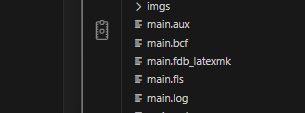
\includegraphics[width=11cm]{imgs/image.png}
    \caption{Example figure}
    \label{fig:example}
\end{figure}
\FloatBarrier

\section{Results}
Your results go here.

\section{Conclusion}
Summary and conclusions.

\begin{table}[H]
\centering
\caption{Table Title Here}
\label{tab:your-label}
\begin{tabular}{p{4cm} c}
    \toprule[1pt]
    \textbf{Frequency Band [GHz]} & \textbf{Purpose} \\ \midrule
    \textcolor{blue}{XX.XX -- XX.XX} & \textcolor{blue}{Description of purpose} \\
    XX.XX -- XX.XX                 & Description of purpose \\
    XX.XX -- XX.XX                 & Description of purpose \\
    XX.XX -- XX.XX                 & Description of purpose \\
    XX.XX -- XX.XX                 & Description of purpose \\
    XX.XX -- XX.XX                 & Description of purpose \\
    XX.XX -- XX.XX                 & Description of purpose \\
    XX.XX -- XX.XX                 & Description of purpose \\
    \bottomrule[1pt]
\end{tabular}
\end{table}


Here is a citation test \cite{latex2020}.


\printbibliography

\end{document}